\documentclass[12pt,a4paper]{article}
\usepackage[english]{babel}
\usepackage{authblk, amsmath, graphicx}
\usepackage{natbib}
\usepackage{listings}
\usepackage{caption, float, subfigure}
\usepackage{adjustbox}
\usepackage{placeins}
\usepackage{booktabs, caption}
\usepackage[table, xcdraw]{xcolor}
\usepackage{titling, lipsum}
\usepackage{tablefootnote}
\usepackage{array}
\usepackage{tcolorbox}
\tcbuselibrary{minted,breakable,xparse,skins}

\captionsetup{
    labelfont=bf
}
\definecolor{bg}{gray}{0.95}
\definecolor{lightgray}{rgb}{0.9,0.9,0.9}
\DeclareTCBListing{mintedbox}{O{}m!O{}}{%
  breakable=true,
  listing engine=minted,
  listing only,
  minted language=#2,
  minted style=default,
  minted options={%
    linenos,
    gobble=0,
    breaklines=true,
    breakafter=,,
    fontsize=\footnotesize,
    numbersep=8pt,
    #1},
  boxsep=0pt,
  left skip=0pt,
  right skip=0pt,
  left=25pt,
  right=0pt,
  top=3pt,
  bottom=3pt,
  arc=5pt,
  leftrule=0pt,
  rightrule=0pt,
  bottomrule=2pt,
  toprule=2pt,
  colback=bg,
  colframe=lightgray,
  enhanced,
  overlay={%
    \begin{tcbclipinterior}
    \fill[lightgray] (frame.south west) rectangle ([xshift=20pt]frame.north west);
    \end{tcbclipinterior}},
  #3}

\newcolumntype{L}[1]{>{\raggedright\arraybackslash}p{#1}}
\newcolumntype{C}[1]{>{\centering\arraybackslash}p{#1}}

% setting of the Table of Contents
\usepackage{tocloft}
\renewcommand{\cftsecleader}{\cftdotfill{\cftdotsep}}

% Guide for formatting I suppose
\renewcommand{\baselinestretch}{1.5}
\usepackage[left=3cm,right=2cm,top=2cm,bottom=2cm]{geometry}

%\usepackage[flushleft]{threeparttable}


\definecolor{bonnblue}{RGB}{0,79,158} % RGB values for #004F9E

\usepackage[colorlinks=true, linkcolor=black, urlcolor=bonnblue, citecolor=bonnblue]{hyperref}



\begin{document}

\begin{titlepage}
    \begin{center}
        \vspace*{2cm}
            
        \LARGE
        \textbf{Global Real Interest Rate Dynamics and Monetary Policy Announcements}
            
        \vspace{3cm}

        \large
        Master Thesis Presented to the \\ Department of Economics at the \\
        Rheinische Friedrich-Wilhelms-Universität Bonn

        \vspace{1.5cm}

        In Partial Fulfillment of the Requirements for the Degree of \\
        Master of Science (M.Sc.)

        \vfill

        Supervisor: Janko Heineken, Farzad Saidi

        \vspace{1cm}

        Submitted in August 2024 by:\\
        Alper Yıldırım \\
        Matriculation Number: 50075931
            
    \end{center}
\end{titlepage}

% ============================================================
\renewcommand*\contentsname{Table of Contents}
\tableofcontents
\thispagestyle{empty}

\newpage
\setcounter{page}{1}

\begin{quote}
    \itshape
    \setlength{\leftskip}{1cm}
    By providing long-run guidance, the central bank may influence long-term interest rates. \\
    \normalfont
    \hspace*{\fill}--- Isabel Schnabel, Member of the Executive Board of the ECB
\end{quote}

\section{Introduction}

The declining trend of the interest rates in the past 50 years is striking. Although some authors discussed that the secular decline can be traced back for centuries. \citep{rogoff2022} In a recent study, \citet{hillenbrand2022} found that a 3-day time windows around the Federal Open Market Committee (FOMC) meetings capture the secular decline in 10-year Treasuries in the past few decades, and outside-window yield changes are transitory. In the face of this research, the natural question that arises is the following: Can the monetary policy decisions of central banks other than the Fed explain the change in long-term national bond yields, by providing a kind of ``long-term forward guidance'', or is this a unique case for the Fed? Furthermore, in relation to ``Global Financial Cycle" research \citep{miranda2020us, rey2021}, can the secular decline in other national long-term bond yields be accounted by the Fed's monetary policy decisions?

\section{Related Literature}

The decline in real interest rates in recent decades is noted by \citet{summers2014reflections}, claiming that the lack of investment opportunities along with raised private saving propensities and reduced investment propensities. That is to say, this approach determines a macroeconomic framework around the Global Financial Crisis and the Eurozone crisis. On the other hand, \citet{rogoff2022} argues that the decline in the long-term real interest rates is not particular to recent decades. Instead, it is a trend stationary and persistent decline that dates back to the 1300s. This long-term decline, according to \citet{rogoff2022} reflects the reduced discount factors over time at the global scale and challenges explanations around productivity and demographics. \\

Shifting the perspective on the decline of real interest rates to financial markets and monetary policy, in their study, \citet{gilchrist2014us} presented that the longer-term interest rates in advanced economies, proxied by 10-year bond yields, were declined in response to both an unanticipated conventional easing and unconventional monetary actions of the Fed. While conventional monetary easing steepens the yield curve in advanced economies through a larger decline in the short-end of the yield curve, unconventional monetary actions narrow the yield spread of nominal foreign interest rates down. Moreover, \citet{hanson2015monetary} documented that the changes in monetary policy affect the 10-year forward real rates, utilizing movements during the FOMC announcement days. They offer a ``reaching for yield'' mechanism such that the yield-oriented investors substitute for longer-term bonds as short-term yields decline if the yield curve is upward-sloping. In turn, increasing demand for longer maturity bonds leads to increasing prices and declining yields. That is, this explanation relies on a ``term premium'' effect. \citep{hanson2015monetary}\\

% Add a few studies similar to Gilchrist and Hanson


Starting from \citet{romer2004new} and \citet{gurkaynak2005}, there is a growing literature on identifying high-frequency monetary policy shocks. \citet{nakamura2018high} provide a comprehensive analysis of the ``Fed information effect'' and monetary non-neutrality by examining high-frequency interest rate changes around FOMC meetings, i.e., monetary policy announcements influence not only financial variables but also adjust the beliefs and expectations of private sector participants about economic trajectory. By incorporating the adjustment of private sector expectations, the authors reveal that a considerable portion of the observed responses in real interest rates can be attributed to changes in perceptions of the natural rate of interest, emphasizing the dual role of monetary policy in shaping expectations. Yet, later on, \citet{bauer2023alternative} challenge the prevailing "Fed information effect" hypothesis, which posits that monetary policy announcements convey new information about economic conditions to the market. By analyzing high-frequency financial data around FOMC meetings and incorporating public economic news in their regressions, they propose the "Fed response to news" hypothesis. Their findings suggest that both the Fed and market participants react similarly to public economic information rather than the Fed possessing unique, market-moving insights. \\

% hillenbrand'ı kopyala yapıştır yaptım
\citet{hillenbrand2022} states that a narrow window around Fed meetings captures the secular decline in U.S. Treasury yields since 1980. Yield movements outside this window are transitory and wash out over time. This is surprising because the forces behind the secular decline are thought to be independent of monetary policy. However, Fed announcements might provide guidance about the long-run path of interest rates. In direct support of such“Long-run Fed Guidance”. \\

Heretofore, I discussed the literature on the monetary policy and declining real interest rates, depicted in bond yields. Nevertheless, another line of research that is indispensable for this study, is on the ``Global Financial Cycle'', which is elaborated in \citet{miranda2015world}, \citet{miranda2020us} and \citet{rey2021}. \citet{miranda2020us} demonstrated that a single global factor explains around one-fifth of a common variation of the risky asset prices around the world. Given that the U.S. dollar is the dominant currency of global banking, one instance of this is that almost \%80 of the syndicated loans that have an average amount greater than \$5 million are denominated in the U.S. dollar, the monetary policy decisions by the Fed have a direct impact over the Global Financial Cycle. The potential explanations for this phenomenon are the deleveraging of the financial intermediaries around the globe, and relatedly, a decline in global credit and gross capital flows, and a significant rise in aggregate risk aversion. \citep{miranda2020us} In their work on surrender options in life insurance and market interest rates, \citet{kubitza2023life} estimates two-stage least-squares regressing German government bond rates on the U.S. monetary policy shocks, claiming a transmission through the international bond market channel.


\section{Data and Institutional Background}

\subsection{Eurozone}

The Governing Council is the principal decision-making entity of the European Central Bank (ECB) for conducting monetary policy. The Governing Council consists of twenty-six members---six members of the Executive Board and the Euro-area national central bank governors. While the Governing Council members meet twice a month in order to evaluate macroeconomic and financial conditions, it decides monetary policy stance in every six weeks. The Governing Council conducts monetary policy through three key interest rates: the main refinancing operations rate, the deposit facility rate and the marginal lending facility rate. I obtained the dates of monetary policy decisions from the ECB website. My sample contains in total 299 monetary policy decision dates, from March 1999 to March 2024. \\

I collected yield data on European bonds, which includes \textit{nominal} interest rates of the AAA-rated government bonds, using the ECB Data Portal. The term structure data is modeled with the Svensson model, i.e., this data offers zero-coupon continuously-compounded yield curve.

\subsection{United Kingdom}

The Monetary Policy Committee (MPC) is the key decision-making body of the Bank of England (BoE) to conduct monetary policy. The MPC is made up of nine members – the Governor, the three Deputy Governors for Monetary Policy, Financial Stability and Markets and Banking, our Chief Economist and four external members appointed directly by the Chancellor. The main monetary policy interest rate set by the MPC is called `Bank Rate', which refers to the interest rate BoE pay to commercial banks that hold money with the BoE. I collected yield data of UK government bonds, also known as gilts, from XXXX to XXXX from the BoE database. Similarly, the yield data contains estimation for zero-coupon continuously-compounded yields. \citet{anderson2001new}

\subsection{Switzerland}
% copy paste hepsi https://www.snb.ch/en/the-snb/mandates-goals/monetary-policy
The Governing Board is the SNB's highest management and executive body. Its three members are appointed for a six-year term by the Federal Council on the recommendation of the Bank Council. The Governing Board is responsible, in particular, for monetary policy. The Swiss National Bank implements its monetary policy by setting the SNB policy rate. In so doing, it seeks to keep the short-term Swiss franc money market rates close to the SNB policy rate. These yields are known as spot interest rates, i.e. yields on zero-coupon bonds. Spot interest rates and/or the maturity/interest rate structure are estimated using the extended Nelson/Siegel procedure.

\subsection{Japan}
% copy paste https://www.boj.or.jp/en/mopo/outline/index.htm
The basic stance for monetary policy is decided by the Policy Board at Monetary Policy Meetings (MPMs). At MPMs, the Policy Board discusses the economic and financial situation, decides the guideline for money market operations and the Bank's monetary policy stance for the immediate future, and announces decisions immediately after the meeting concerned.

\subsection{Australia}

The Reserve Bank Board is the key decision-making body of the Reserve Bank of Australia. The Reserve Bank Board consists of nine members, of which at least five (including the Governor as Chair or Deputy Governor as Deputy Chair) must be present to conduct a meeting. The Board meets eight times a year. The Reserve Bank Board operates monetary policy through the `cash rate target', i.e., the interest rate on overnight loans. In sample, dates for the monetary policy decisions are ranged from August 1992 to March 2024, and in total, there are 215 meetings. Similarly, I collected yield data of Australian government bonds from July 1992 to May 2013 from the Reserve Bank of Australia's database. The data contains estimation for zero-coupon continuously-compounded yields.

\subsection{Canada}

\citet{bolder2004empirical} constructed the historical zero-coupon yield curve data.

\section{The Decline in Interest Rates and Monetary Policy}

In the selected sample of advanced economies, the results imply heterogeneous effects of the national monetary policy and the U.S. monetary policy. Furthermore, unconventional monetary policy interventions, e.g., quantitative easing programs, yield varying results in different countries. Therefore, I examine the yield movements around the monetary policy decision dates by country.

\subsection{German Bund Yields}

In Figure \ref{fig:german2008} and \ref{fig:german1999}, the cumulative yield change of the 10-year German bunds with respect to both ECB and FOMC announcements is depicted for complete sampled interval and post-crisis period. Figure \ref{fig:german2008} implies that in the post-crisis period, the monetary policy announcements by the ECB appear to be white noise for 10-year German bunds. In contrast, in the pre-crisis period, the yield movements around the ECB monetary policy announcements co-move with the trend. This finding provokes a question of what phenomenon exactly causes this kind of structural break. More specifically, the cumulative yield change and ECB's within-window yield change have almost opposite directions around 2009-2012. Therefore, the effect of the unconventional monetary policy tool of the ECB, namely the Securities Market Programme of 2010-2012, and the effect of the quantitative easing by the Fed are potential causes. Nevertheless, the fragile relationship between the cumulative yield change and ECB's within-window yield and the yield movement is obvious. \\

\begin{figure}[!htbp]
    \centering
    \caption{$\Delta$Yield in 3-days Around the ECB and FOMC Announcements (2008-2024)}   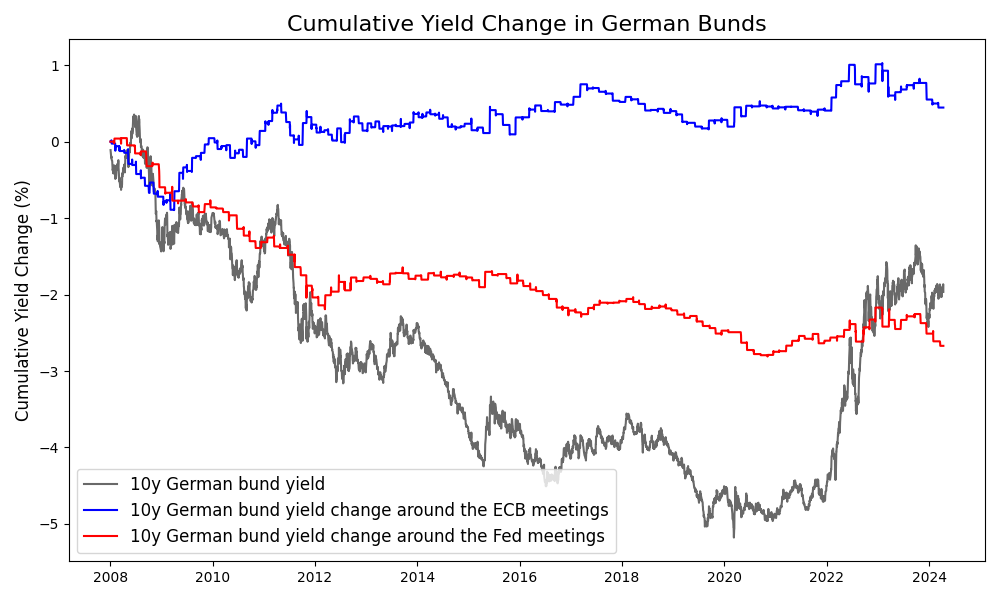
\includegraphics[width=0.9\textwidth]{figures/2008_german_bunds_figure1a.png}
    \label{fig:german2008}
\end{figure}

\begin{figure}[!htbp]
    \centering
     \caption{$\Delta$Yield in 3-days Around the ECB and FOMC Announcements (1999-2024)}   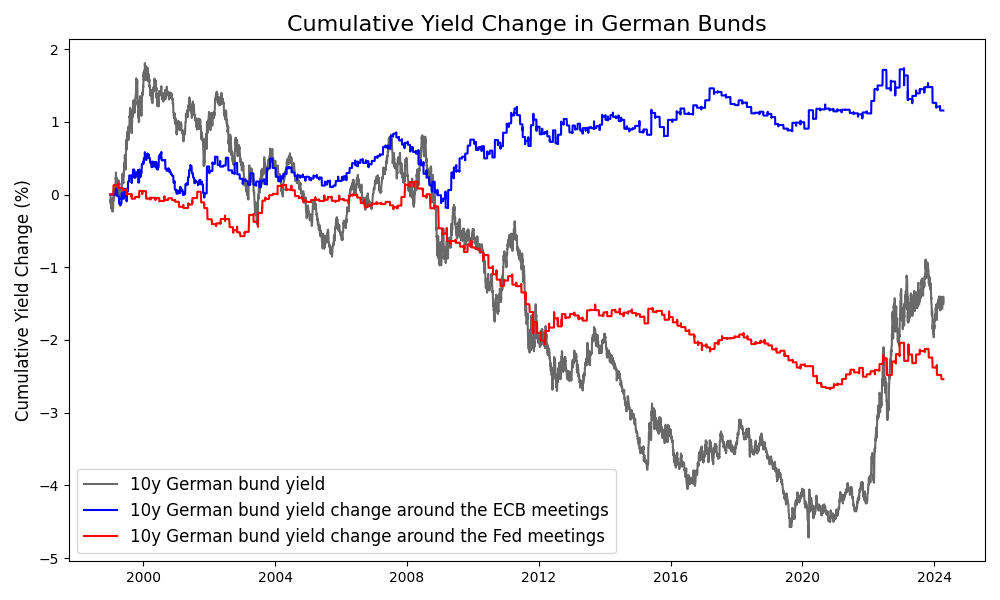
\includegraphics[width=0.9\textwidth]{figures/1999_german_bunds_figure1a.png}

    \label{fig:german1999}
\end{figure}


On the other hand, the yield movements of 10-year German bunds around the FOMC announcements have stronger co-movement with the trend in the whole sample. However, it is important to note that there was a jump around 2012 in this co-movement but the co-movement remained persistent even after that jump. As in the case of the ECB announcements, the question arises as to what caused that jump with potential explanations of the unconventional monetary policy tools. Using a straightforward OLS approach to measure the cross-border monetary policy spillovers from the FOMC announcements to German bunds, I regress the yield change of 10-year German bunds on the yield change of 10-year Treasuries around the 3-day FOMC announcements:

\begin{equation} \notag
    \Delta 10yr_{t-1,t,DE}= \beta_0 + \beta_1\, \Delta 10yr_{t-1,t,US} + \varepsilon_t
\end{equation}
\vspace{-0.25cm}

The results of the spillover regression is depicted in Table \ref{tab:spillreg} and Figure \ref{fig:spillovers}. The estimation to assess the magnitude of cross-border spillovers from 10-year Treasury yields to 10-year German bunds indicates that a one standard deviation change in U.S. Treasury yields corresponds to a 0.44 standard deviation change in German bund yields, highlighting the significant influence of FOMC announcements on German bond markets.


% ======================================

\subsection{UK Gilt Yields}

Figure \ref{fig:uk1999} depicts the yield change of the 10-year government bonds of the United Kingdom, gilts namely, with respect to both BoE and FOMC announcements for both sample intervals, i.e., post-1999 and post-crisis. The simple descriptive evidence suggests a divergence between the German bunds and the UK gilts. That is, neither in pre-crisis nor post-crisis periods, the effect of the BoE's rate announcements became white noise. Instead, regardless of the selected time interval, the yield movements around the BoE and FOMC announcements accounts for the yield movement itself. To see this strong relationship, the yield changes around both meetings are combined in Figure \ref{fig:uk1999both}. \\

Moreover, in contrast to other countries in the sample, the fact that the decline in bond yields could be explained by the decline in the 3-day windows around the BoE's decisions may indicate that the BoE, unlike other central banks in the sample, enjoys relatively stronger monetary authority and a certain degree of autonomy in the face of the Global Financial Cycle. While the UK's divergence from other countries requires a more in-depth macroeconomic analysis, the fact that the 3-day windows around the BoE and FOMC announcements explain the decline in long-term bond yields confirms that, contrary to conventional thinking, monetary policy is likely to explain the decline in long-term interest rates. Lastly, the result of regressions yield change of 10-year UK gilts on the yield change of 10-year Treasuries around the 3-day FOMC windows indicate that for one standard deviation decline in the 10-year Treasuries is associated with 0.49 standard deviation decline in the 10-year UK gilts, confirming the cross-border monetary spillovers.

\begin{figure}[!htbp]
    \centering
    \caption{$\Delta$Yield in 3-days Around the BoE and FOMC Announcements (1999-2024)}    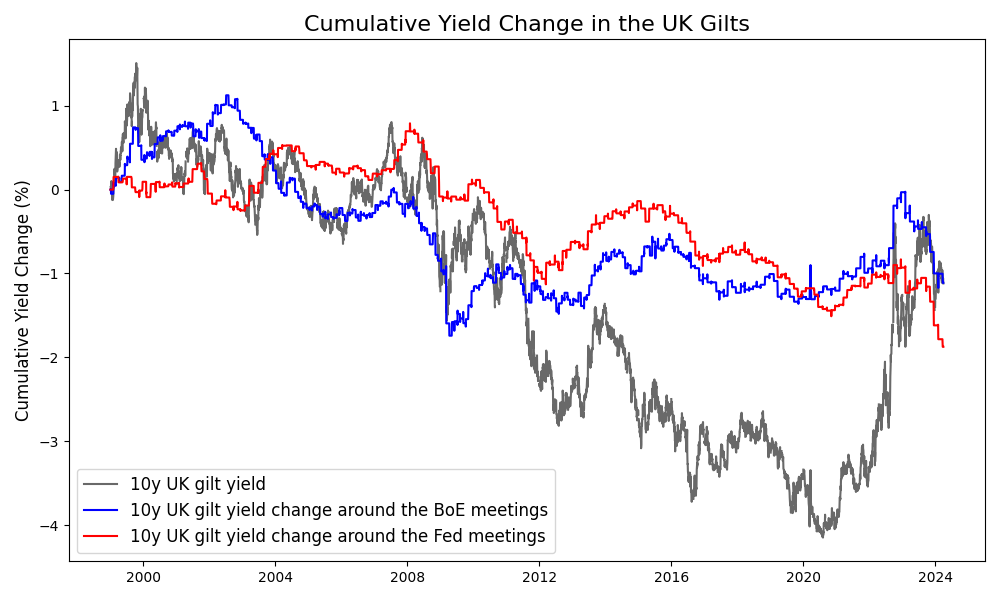
\includegraphics[width=0.9\textwidth]{figures/1999_uk_gilts_figure1a.png}
    \label{fig:uk1999}
\end{figure}
\vspace{0.2cm}

\begin{figure}[!htbp]
    \centering
    \caption{$\Delta$Yield in 3-days Around the Both CBs' Announcements (1999-2024)}    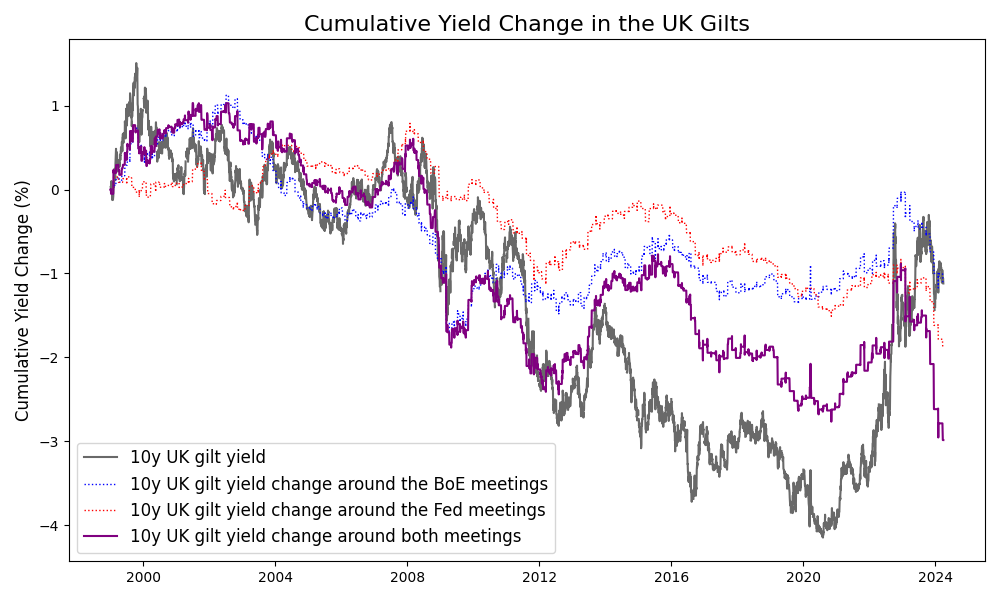
\includegraphics[width=0.9\textwidth]{figures/1999_uk_gilts_figure1a_combined.png}

    \label{fig:uk1999both}
\end{figure}


% ======================================

\subsection{Japanese Government Bond (JGB) Yields}

Figure \ref{fig:boj1997} illustrate the yield movements of 10-year Japanese Government Bonds (JGBs) including 3-day time window change with respect to the FOMC and BoJ announcements, for both post-1997 and post-crisis intervals. In line with the findings in the Germany case, it is evident that there was a striking structural break around the Global Financial Crisis. A more thorough analysis shows that the break occurred approximately between 2006 and 2008. From 1997 until the Global Financial Crisis, the 3-day yield windows built around the BoJ announcements captured the change in bond yields to a large degree and in tandem with the trend, whereas in the post-crisis period, the change in bond yields became insensitive to BoJ announcements. On the other hand, as shown in Figure \ref{fig:boj1997}, the 3-day windows around the FOMC announcements in the post-crisis period largely account for the change in bond yields. To observe this pattern more precisely, see Figure \ref{fig:boj97mix}, which depicts the time windows around the BoJ announcements in the pre-crisis period and the time windows around the FOMC in the post-crisis period. Additionally, the coefficient for the cross-border monetary spillover regression, presented in Table \ref{tab:spillreg} and Figure \ref{fig:spillovers}, illustrates that at the 0.05 significance level, the decline in the U.S. Treasuries spills over the Japanese long-term government bonds. In terms of economic significance, for one standard deviation decline in the U.S. Treasuries lead 0.1 standard deviation decline in Japanese bonds.\\

\begin{figure}[!htbp]
    \centering
     \caption{$\Delta$Yield in 3-days Around the BoJ and FOMC Announcements (1997-2024)}   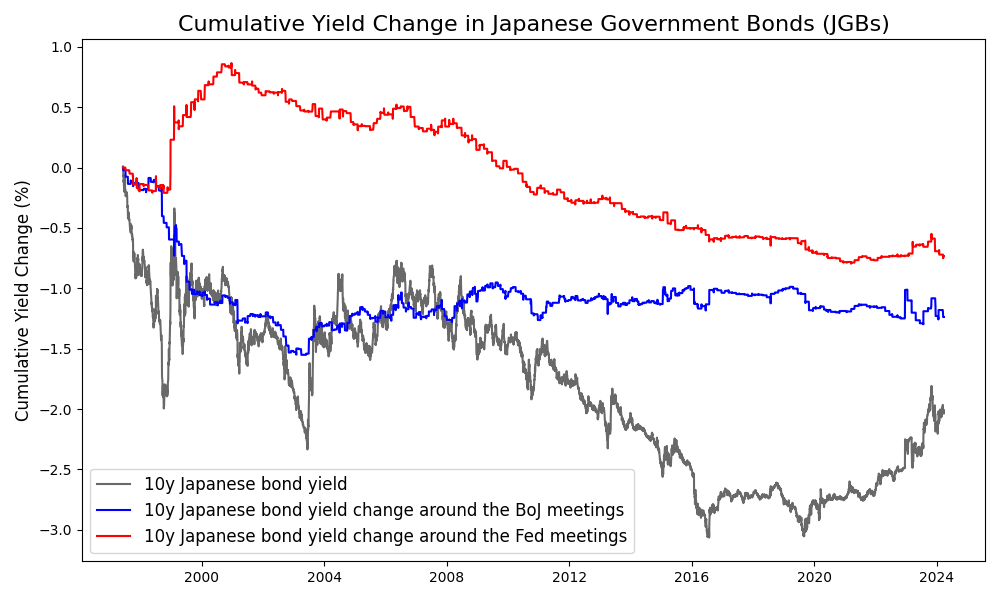
\includegraphics[width=0.9\textwidth]{figures/1997_japanese_bonds_figure1a.png}

    \label{fig:boj1997}
\end{figure}

While on the one hand, the patterns of this change brought about by the Global Financial Crisis are evident and raise the question of the amplification of the Global Financial Cycle, on the other hand, questions remain about the impact of unconventional monetary policy tools on this outcome. As in the case of Germany, the ECB's Securities Market Program of 2010-2012 is being discussed, whether the Japanese QE program, which ended in 2006, had an impact on this structural break remains a noteworthy research agenda.



\begin{figure}[!htbp]
    \centering
    \caption{$\Delta$Yield Around the Altered BoJ-FOMC Announcements (1997-2024)} 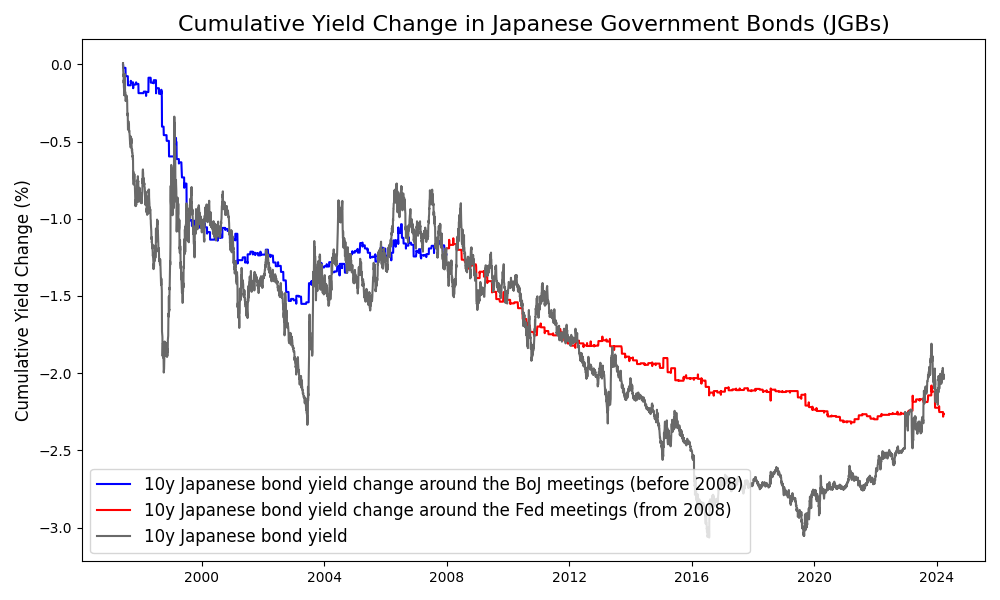
\includegraphics[width=0.9\textwidth]{figures/1997_japanese_mixed.png}

    \label{fig:boj97mix}
\end{figure}

% ======================================

\subsection{Canadian Bond Yields}

Due to spatial proximity and entangled economic and financial relationships, Canada has a particular status in the sample. Employing a global VAR model, \citet{beaton2011financial} emphasizes the significance of financial variables in transmission of shocks from the U.S. to Canada, including both disturbances to real economic activity and to financial conditions. Financial linkage, combined with robust trade relations and geographical proximity, would be likely spillovers from the U.S. monetary policy decisions to Canadian economy and to Canadian bond yields in particular. Indeed, in both the post-1999 and post-crisis sample, depicted in Figures \ref{fig:canada2008} and \ref{fig:boc1999}, it is obvious that Canadian bond yield movements in the 3-day time windows of the FOMC announcements account for the overall trend in Canadian bond yields. As deep-rooted economic entanglements might suggest, there is no evident structural break per se around the Global Financial Crisis that intensified the evidence for the Global Financial Cycle.

\begin{figure}[!htbp]
    \centering
    \caption{$\Delta$Yield in 3-days Around the BoC and FOMC Announcements (2008-2024)}
    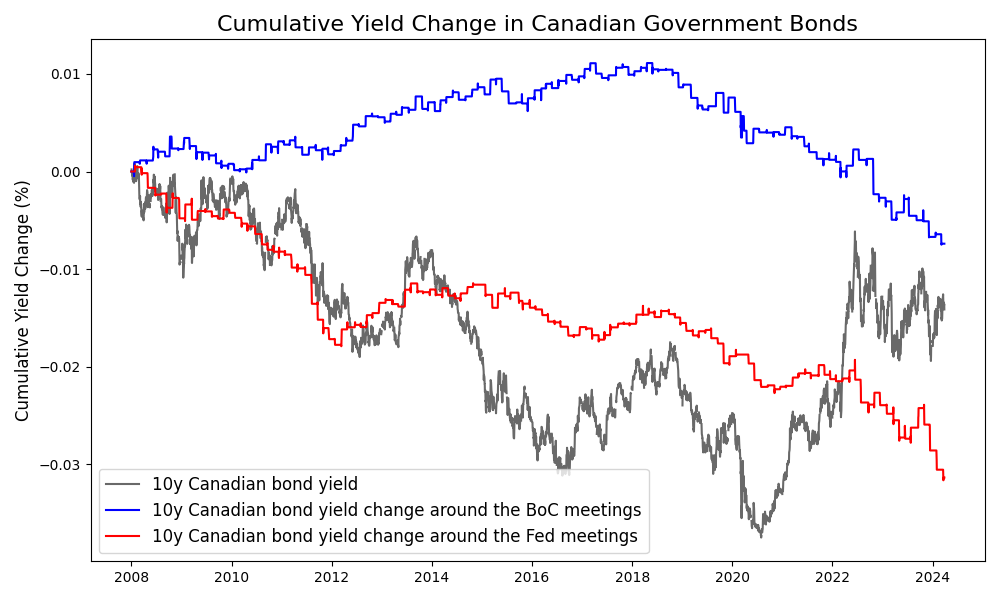
\includegraphics[width=\textwidth]{figures/2008_canadian_bond_figure1a.png}
    \label{fig:canada2008}
\end{figure}


\begin{figure}[!htbp]
    \centering
    \caption{$\Delta$Yield in 3-days Around the BoC and FOMC Announcements (1999-2024)}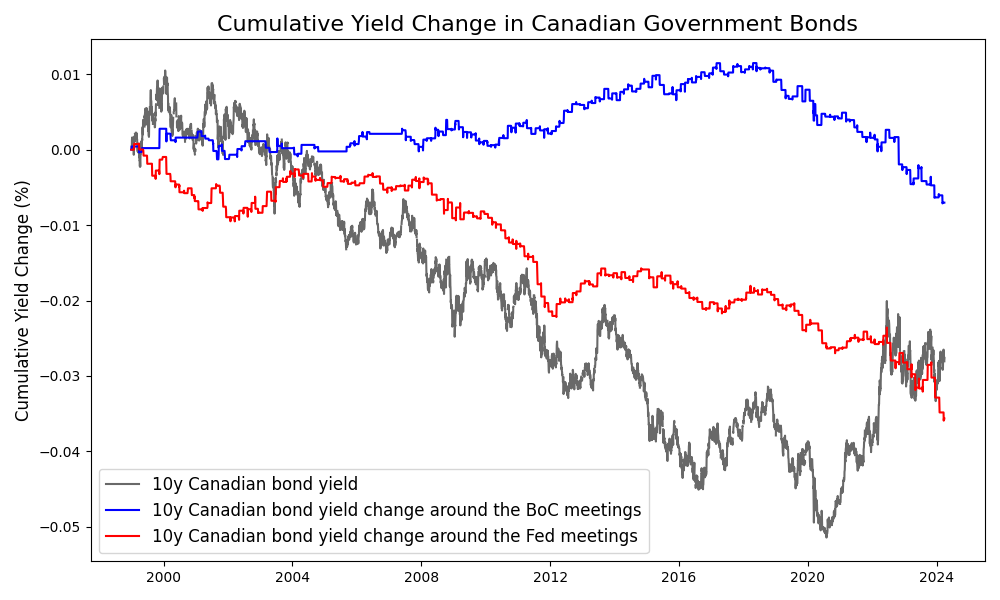
\includegraphics[width=0.9\textwidth]{figures/1999_canadian_bond_figure1a.png}

    \label{fig:boc1999}
\end{figure}

Using the cross-border spillover regressions as in the previous cases, the results are particularly striking. Illustrated in Table \ref{tab:spillreg}, 100 basis points decline in the U.S. Treasuries is associated with 59 basis points decline in the long-term Canadian bonds around the 3-day FOMC announcement windows, and this result is statistically significant at the 0.01 level. Standardizing for the results, for one s.d. change in U.S. Treasuries is associated with 0.81 change in Canadian bond yields.

\subsection{Swiss Confederation Bond Yields}

Figure \ref{fig:snb2008} and \ref{fig:snb2000} accurately indicate that neither the 3-day windows around the FOMC meetings nor those around the Swiss National Bank meetings have any explanatory power of declining long-term yields. Furthermore, there exist no structural breaks attributable to the Global Financial Crisis. This descriptive result is partly supported by the cross-border spillover regression. In the Column 5 of Table \ref{tab:spillreg}, for 100 basis points decline in the U.S. Treasuries, the yield change in the 10-year Swiss Confederation Bonds is 10.5 basis points. Given that these results differ significantly from those of other countries in the sample, further investigation is warranted. \\

There are significant macro-financial differences between Switzerland and the rest of the sample. First, the statistics and \citet{cwik2024fx} suggest that the Swiss National Bank conducts sizeable currency intervention in order to influence inflation or to protect the ``safe haven'' status of the Swiss Franc. Further, \citet{bacchetta2022understanding} states that the exchange rate affects the real interest rates in Switzerland, through the convenience yield, mediated by a valuation effect.


\subsection{Australian Government Bond Yields}

Figures \ref{fig:rba2008} and \ref{fig:rba1997} exhibit a overview compared to the previous figures. This is mainly because neither the Fed's nor the RBA's 3-day monetary policy decision windows seem to have much impact on 10-year bond yield changes. Indeed, if observing the trend, the bond yield movement in the RBA decision windows is in the opposite direction to the trend in bond yields. On the other hand, even if the Fed's influence on bond movements is less than in other cases such as Canada or Germany, there is a noticeable co-movement, especially in certain sub-time periods. Nevertheless, this weak and ineffectual co-movement can only account for a too little portion of the variation. For the spillovers around the 3-day FOMC announcement windows, the explained variation of this regression is restricted to 0.009, while the standardized coefficient suggests that for a one standard deviation decline in the U.S. Treasuries, the decline in the Australian Government Bonds is only 0.096 standard deviation. 

\begin{figure}[!htbp]
    \centering
     \caption{$\Delta$Yield in 3-days Around the SNB and FOMC Announcements (2008-2024)}   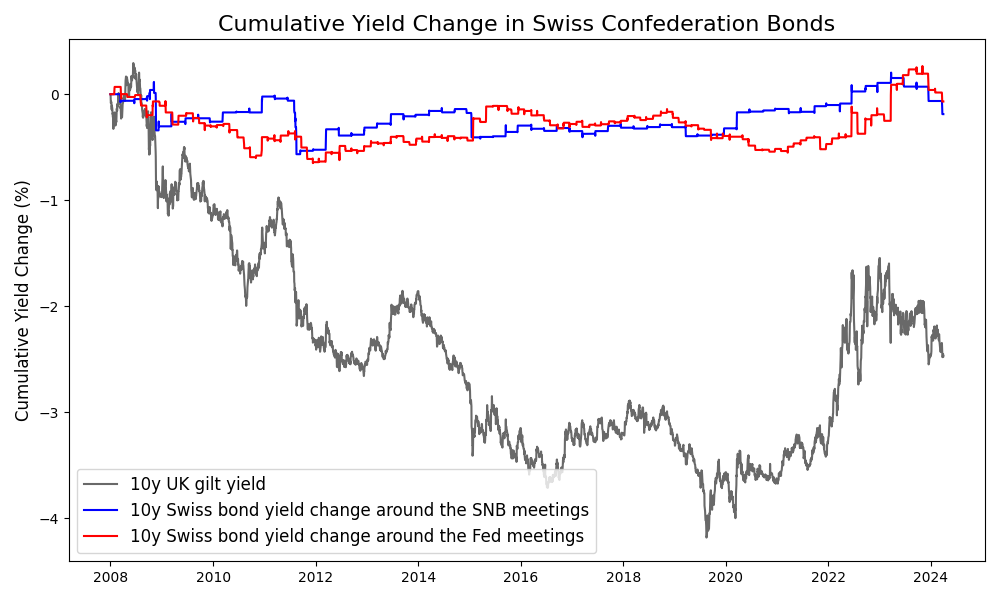
\includegraphics[width=0.9\textwidth]{figures/2008_swiss_bonds_figure1a.png}

    \label{fig:snb2008}
\end{figure}

\begin{figure}[!htbp]
    \centering
    \caption{$\Delta$Yield in 3-days Around the SNB and FOMC Announcements (2000-2024)}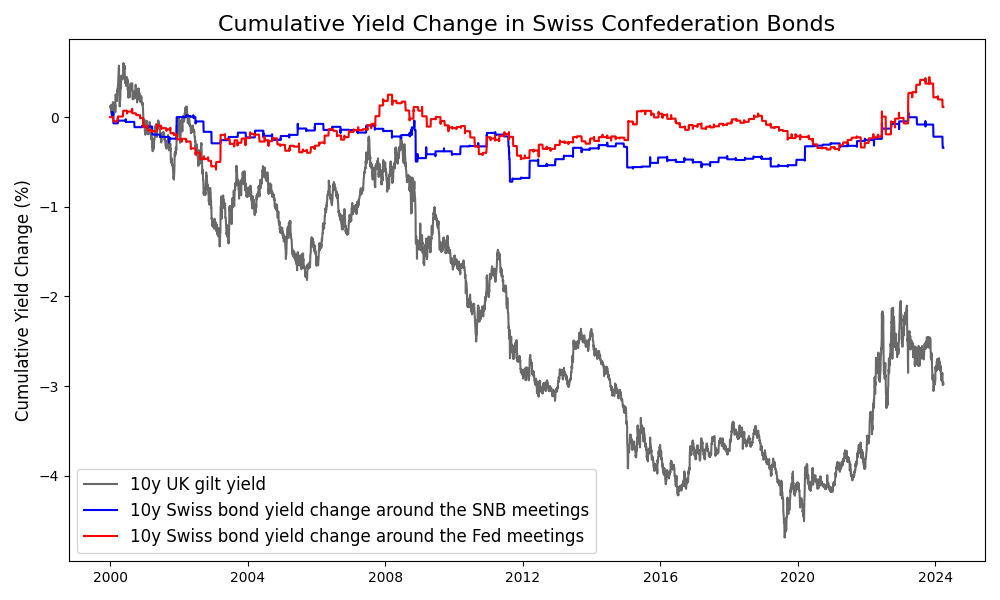
\includegraphics[width=0.9\textwidth]{figures/2000_swiss_bonds_figure1a.png}

    \label{fig:snb2000}
\end{figure}

\FloatBarrier

% ======================================


\begin{figure}[!htbp]
    \centering
    \caption{$\Delta$Yield in 3-days Around the RBA and FOMC Announcements (2008-2024)}    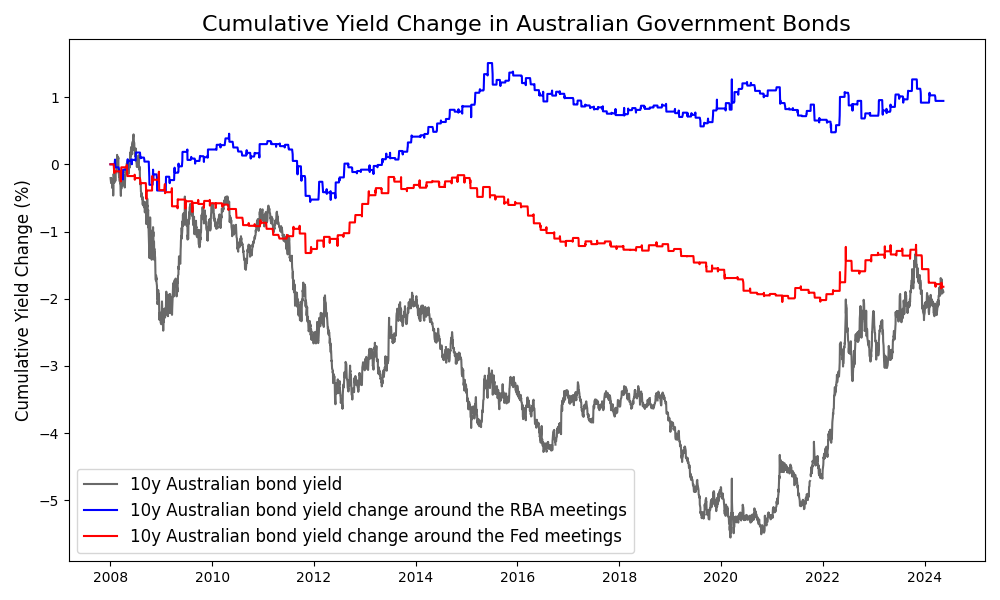
\includegraphics[width=0.9\textwidth]{figures/2008_australian_bonds_figure1a.png}

    \label{fig:rba2008}
\end{figure}

\begin{figure}[!htbp]
    \centering
    \caption{$\Delta$Yield in 3-days Around the RBA and FOMC Announcements (1997-2024)}    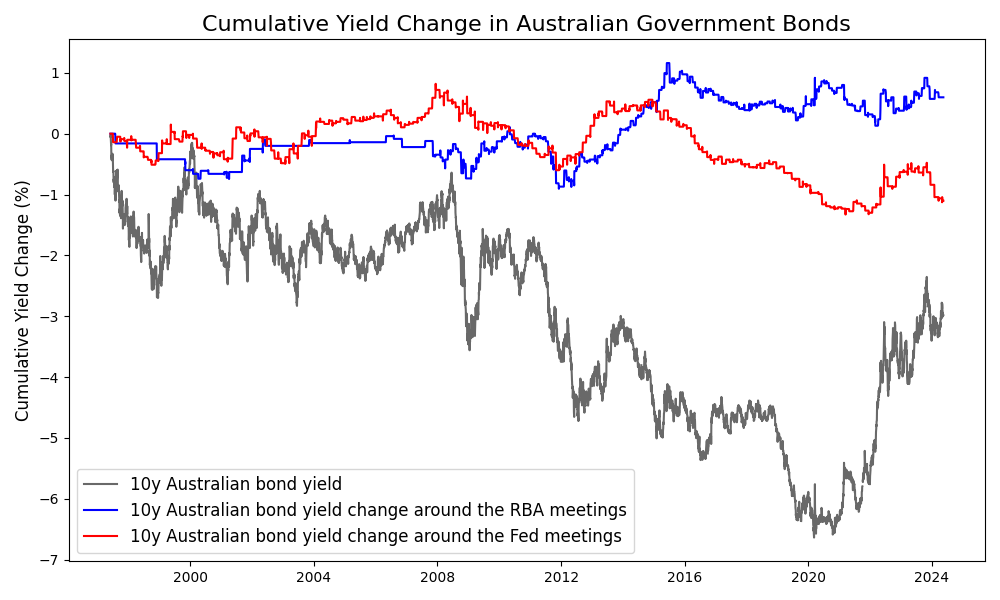
\includegraphics[width=0.9\textwidth]{figures/1997_australian_bonds_figure1a.png}

    \label{fig:rba1997}
\end{figure}

\newpage
% ======================================

\begin{figure}[!htbp]
    \caption{Spillovers from 10yr Treasury to Government Bonds Around FOMC Meetings}
    \centering
    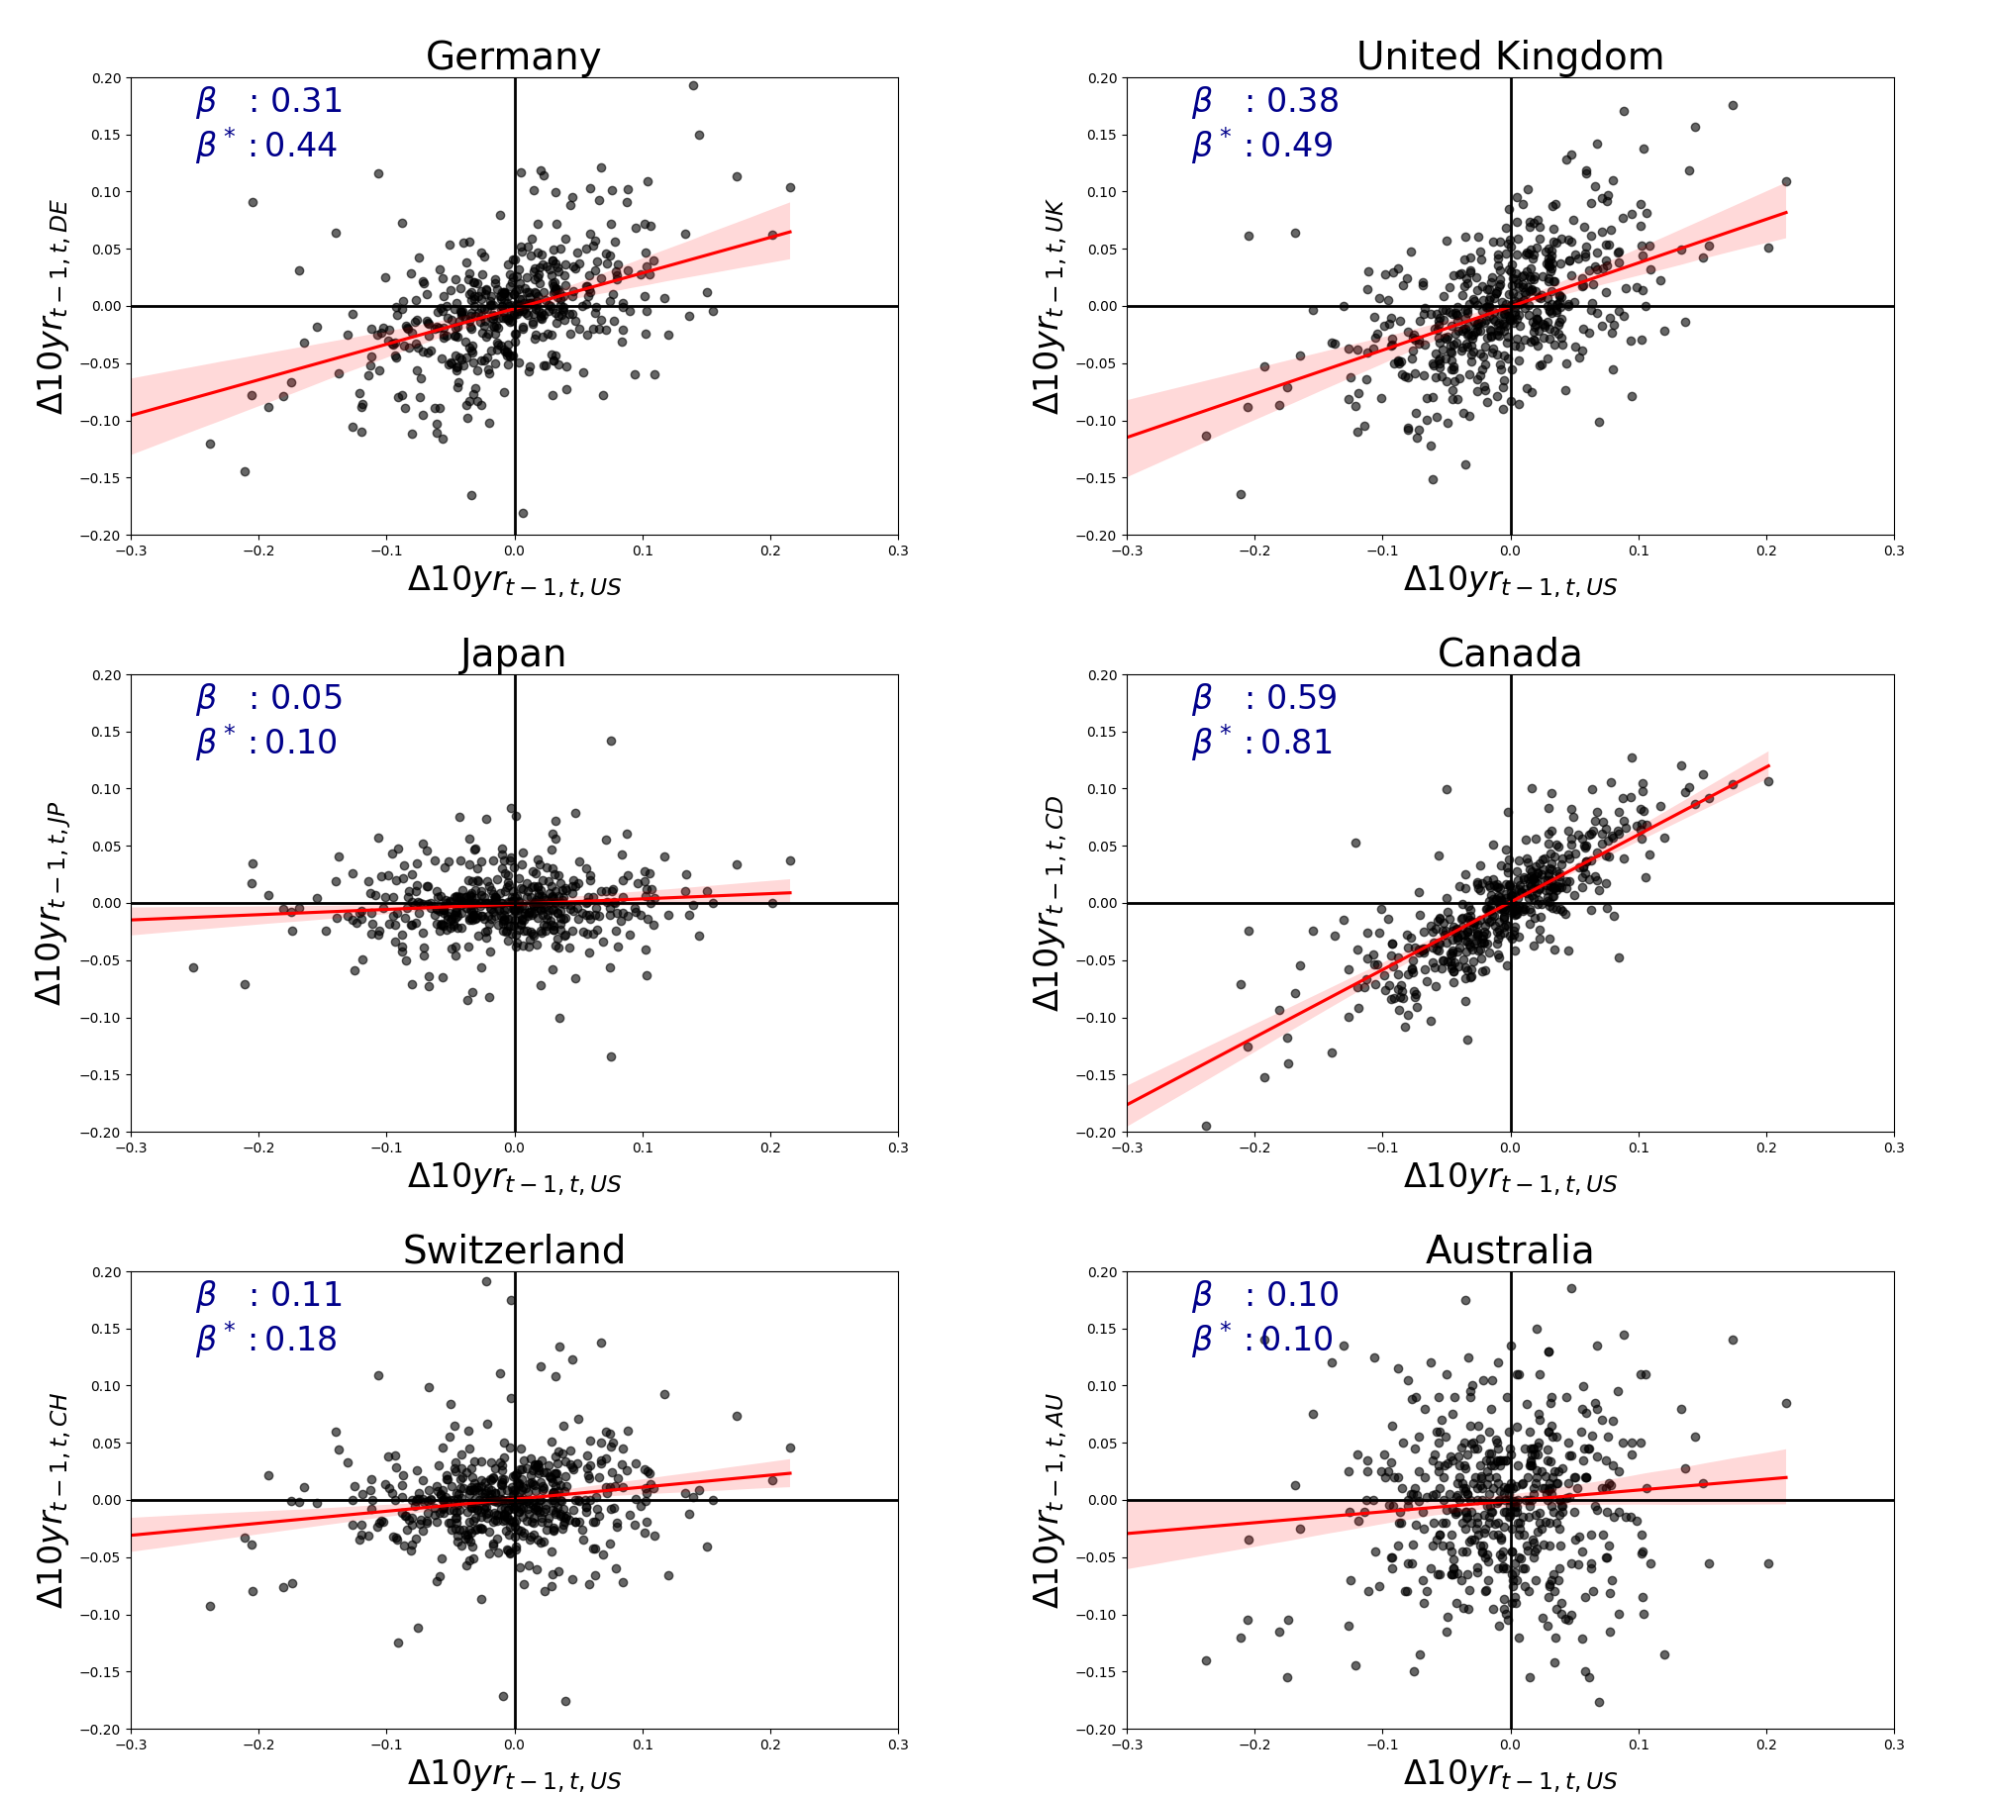
\includegraphics[width=\textwidth]{figures/bondspillovers.png}
    \label{fig:spillovers}
\end{figure}

\begin{table}[!htbp]
\caption{Spillovers from 10yr Treasury to Government Bonds Around FOMC Meetings}
\centering
\begin{tabular}{lcccccc}
\toprule
& \multicolumn{6}{c}{$\Delta$10yr_{Home}} \\
\cmidrule(lr){2-7}
& \multicolumn{1}{c}{Germany} & \multicolumn{1}{c}{UK} & \multicolumn{1}{c}{Japan} & \multicolumn{1}{c}{Canada} & \multicolumn{1}{c}{Switzerland} & \multicolumn{1}{c}{Australia} \\
\midrule
$\Delta$10yr_{US} & 0.311$^{***}$ & 0.382$^{***}$ & 0.046$^{**}$ & 0.591$^{***}$ & 0.105$^{***}$ & 0.095$^{**}$ \\
& (0.029) & (0.030) & (0.021) & (0.019) & (0.024) & (0.043) \\
Std. $\Delta$10yr_{US} & 0.44 & 0.49 & 0.1 & 0.813 & 0.182 & 0.095 \\
\midrule
Observations & 477 & 523 & 494 & 482 & 543 & 535 \\
$R^2$ & 0.193 & 0.241 & 0.010 & 0.661 & 0.033 & 0.009 \\
\bottomrule
\end{tabular}
\label{tab:spillreg}
\end{table}


\section{Empirical Strategy}

In the previous section, I demonstrated the compelling fact that the 3-day windows around the FOMC meetings capture the decline of the interest rates for some of the selected advanced economies, more effectively than the 3-day monetary policy decision window of the national central banks. While this descriptive evidence suggest that the effect of the narrow time windows around the Fed decisions can explain the yield declines of advanced economies, to establish a causal link, a further empirical specification is required. To enhance the robustness of the causal link, I incorporated financial frictions into the model. Hence, the baseline specification is:
$$
\begin{aligned}
\Delta_{t-1,t}10\textrm{yr}_i &= \beta_0\;+\;\beta_1\,\textrm{D(3d FOMC)}_t\;+\;\beta_2\, \textrm{FXF}_{i,t} \\&\quad +\,\beta_3 \, [\textrm{D(3d FOMC})\,\times\,\textrm{FXF}]_{i,t}\;+ \varepsilon_{i,t}
\end{aligned}
$$
\vspace{-0.25cm}

\noindent where $\Delta_{t-1,t}10\textrm{yr}$ represents the yield change of 10-year government bond from $t-1$ to $t$ for country $i$. The dummy variable, $\textrm{D(3d FOMC)}_t$, for the 3-day FOMC windows takes a value of 1 on the day before, the day of, and the day after the FOMC meeting, and 0 otherwise. $\textrm{FXF}_{i,t}$ denotes the financial frictions in the foreign exchange markets for country $i$ at time $t$, which are measured using the Corwin-Schultz bid-ask spread estimator \citep{corwin2012simple}. I used bid-ask spreads as a proxy to reflect the liquidity conditions in the FX market. The wider spread translates into lower liquidity in the market and higher transaction costs, and particularly, the times of higher uncertainty and financial distress lead deteriorating liquidity and wider bid-ask spreads. For a detailed construction of the Corwin-Schultz estimator, refer to the Appendix. \\

Accounting for financial frictions, I isolate the impact of FOMC meeting windows on yield changes better, distinguishing it from broader market dynamics that could confound the 
results. Moreover, the interaction term between $\textrm{FXF}_{i,t}$ and $\textrm{D(3d FOMC)}_t$ captures the differential effect of the FX market frictions, e.g., liquidity conditions or transaction costs, during the 3-day FOMC announcement windows. Therefore, $\beta_3$ becomes a paramater of interest, providing further insights on the transmission mechanisms of the U.S. monetary policy decisions to global bond markets. Nonetheless, the main threat to the identification is the potential endogeneity of the financial frictions. This endogeneity may arise from simultaneity or bi-directional causality, whereby bid-ask spreads might influence bond yield change and vice versa. Furthermore, as the Corwin-Schultz bid-ask spread estimator, which utilizes daily high and low prices, relies on FX data collected on-the-run, thus contains the risk of measurement error that could also lead to biased estimates. \\

To address these endogeneity concerns, I employ an instrumental variable (IV) approach, specifically using a lagged one-week averaged bid-ask spreads as an instrument. Since the lagged bid-ask spreads reflect past conditions in the FX market, it is assumed to influence current yield changes but remains unaffected by contemporaneous shocks to the yield. This approach helps to mitigate reverse causality and ensures that the spread is appropriately exogenous in the model. Moreover, the lagged spread is strongly correlated with the current spread, making it a valid instrument. To implement this approach, I use the Two-Stage Least Squares (2SLS) regression technique. In the first stage, I regress the bid-ask spread on the instrument and other exogenous variables, as well as the interaction term on the instruments and exogenous variables:

$$
\begin{aligned}
    \widetilde{\textrm{FXF}_t} & = \alpha_0 + \alpha_1 \,\textrm{D(3d FOMC)} + \alpha_2\, Z_t +  + v_t \\
    \widetilde{[\textrm{D(3d FOMC})\times\textrm{FXF}]_{i,t}} &= \gamma_0 + \gamma_1 \textrm{D(3d FOMC)}_t + \gamma_2 [\textrm{D(3d FOMC})\,\times\,\textrm{FXF}]_{i,t} + \gamma_3 Z_t + w_t
\end{aligned}
$$
\vspace{-0.25cm}

\noindent Using the predicted values from the first stage, we then estimate the second-stage regression, where we regress the yield change on these predicted values and the dummy variable for the FOMC meeting window:

$$
\begin{aligned}
\Delta_{t-1,t}10\textrm{yr} &= \beta_0\;+\;\beta_1\,\textrm{D(3d FOMC)}_t\;+\;\beta_2\, \widetilde{\textrm{FXF}_t} \\&\quad +\,\beta_3 \, [\widetilde{\textrm{D(3d FOMC})\times\textrm{FXF}}]_{i,t}\; + \varepsilon_t
\end{aligned}
$$
\vspace{0.25cm}

Hence, while $\beta_1$ parameter is interpreted as the effect of the 3-day Fed decision windows over the yield change of 10-year government bond yields for selected economies, the $\beta_3$ parameter captures the differential effect due to the financial frictions. The result of the 2SLS regression is presented at the (IV) column of Table \ref{tab:output} and \ref{tab:betas}. To ensure the validity of the instrumental variable (IV) approach, I conduct several diagnostic tests that assess the strength and relevance of the instruments used in the model. Testing for the underidentification, the Kleibergen-Paap LM statistic implies that the instruments are not underidentified. Furthermore, due to the potential serial correlation in data-generating process, I do not use the Cragg-Donald Wald F-statistic to test for weak instruments. Instead, using the Kleibergen-Paap rk Wald F-statistic, which requires relatively relaxed assumptions on data-generating process, it is confirmed that the instruments are sufficiently strong, compared to the Stock-Yogo critical values. That is to say, the underidentification and weak instrument concerns are mitigated through the relevant test statistics, i.e., the lagged one-week averaged bid-ask spreads is relevant and has sufficient strength for reliable IV estimates presented in the empirical model.


\section{Results}


\newpage



\section{Conclusion}

The findings of this paper contribute to the research field on the monetary policy announcements, interest rate dynamics, and the global financial cycle. The limited yet striking evidence suggests remarkable but heterogeneous influence of the Fed announcements over the long-term government bond yields of selected advanced economies. In Germany and Canada, for instance, there were significant cross-border monetary spillovers from the Fed announcements to long-term yields. Whereas, in Switzerland and Australia, the Fed effect over the long-term interest rates were substantially restricted. Throughout this paper, several potential explanatory variables to explain the sensitivity of national long-term bond yields to the Fed announcements have been discussed, namely, exchange rate interventions, unconventional monetary policy, and frictions in the FX markets. Nevertheless, except for the FX frictions, data unavailability prevented the research inquiry to explain the causes of varying degrees of spillover effects from being explored in more detail. \\

Although lacking statistical significance, the instrumental variable regression suggests that high transaction costs and low market liquidity have a restraining effect on the spillovers from Fed announcements to the long-term bonds of selected advanced economies. This means that the effect of the financial frictions in the global monetary spillovers could be inquired further. Moreover, a future research agenda could focus on a deeper understanding of the mechanisms underlying heterogeneous responses. For this purpose, a more detailed and extensive dataset of granular financial variables or high-frequency monetary policy shocks should be built. This would allow us to better understand how unconventional policies such as quantitative easing (QE) and exchange rate interventions have an impact on the spillovers from Fed announcements to the interest rates in the government bond markets. This would not only allow us to better understand the dynamics of global long-term real interest rates, but also make a valuable contribution to the discourse on the Global Financial Cycle.

\pagebreak

\bibliographystyle{apalike}
\bibliography{ref}

\newpage

\pagenumbering{roman}
\setcounter{page}{1}

\section*{Appendix}

 \pagebreak

 \noindent \textbf{Statement of Authorship:} \\

 \noindent I hereby confirm that the work presented has been performed and interpreted solely by myself except for where I explicitly identified the contrary. I assure that this work has not been presented in any other form for the fulfillment of any other degree or qualification. Ideas taken from other works in letter and in spirit are identified in every single case.

\end{document}